\section{Implementierung}

\subsection {Inbetriebnahme Greifarm}
Der OMX wird als Bausatz geliefert.
Für die Inbetriebnahme ist daher der Zusammenbau und die Installation der entsprechenden Software nötig.
\subsubsection{Zusammenbau}
Der Bausatz des OMX besteht aus ca.\ 60 Teilen (ohne Schrauben, s.\ Abbildung~\ref{fig:omxparts}).
Einige der mit den Servomotoren mitgelieferten Teile werden dabei nicht benötigt, da der Bausatz des OMX diese auch enthält oder ersetzt (z.B.\ längere Kabel).
Von allen Schrauben wurde außerdem Ersatz mitgeliefert.\\
Der Zusammenbau erfolgte nach der auf der Webseite verfügbaren Bauanleitung VERWEIS ANLEITUNG.
Zu beachten ist, dass hier vorausgesetzt wird, dass den Servos bereits die IDs 11 (Basis des Greifarms) bis 15 (Greifer) zugewiesen wurden.
Dies kann über die Software DYNAMIXEL Wizard{\footnote{VERWEIS ODER LINK}} gemacht werden: die Servos einzeln über das U2D2 (s. Abschnitt {\ref{u2d2}}) an den PC anschließen, die ID setzen und den Servo entsprechend markieren oder die ID merken.
Weiterhin müssen bei den Abdeckungen der Servos 12 und 14 die vorgestanzten Abdeckungen herausgebrochen werden.
Dies ist in der Anleitung leicht zu übersehen.
Weiterhin wird angenommen, dass das Horn der Servos bereits angebracht ist.
Hierbei ist darauf zu achten, dass die Einkerbung an Horn und Servo übereinstimmen.\\
Der komplette Zusammenbau erfolgte in ca. 2,5 Stunden.

\begin{figure}[ht!]
\centering
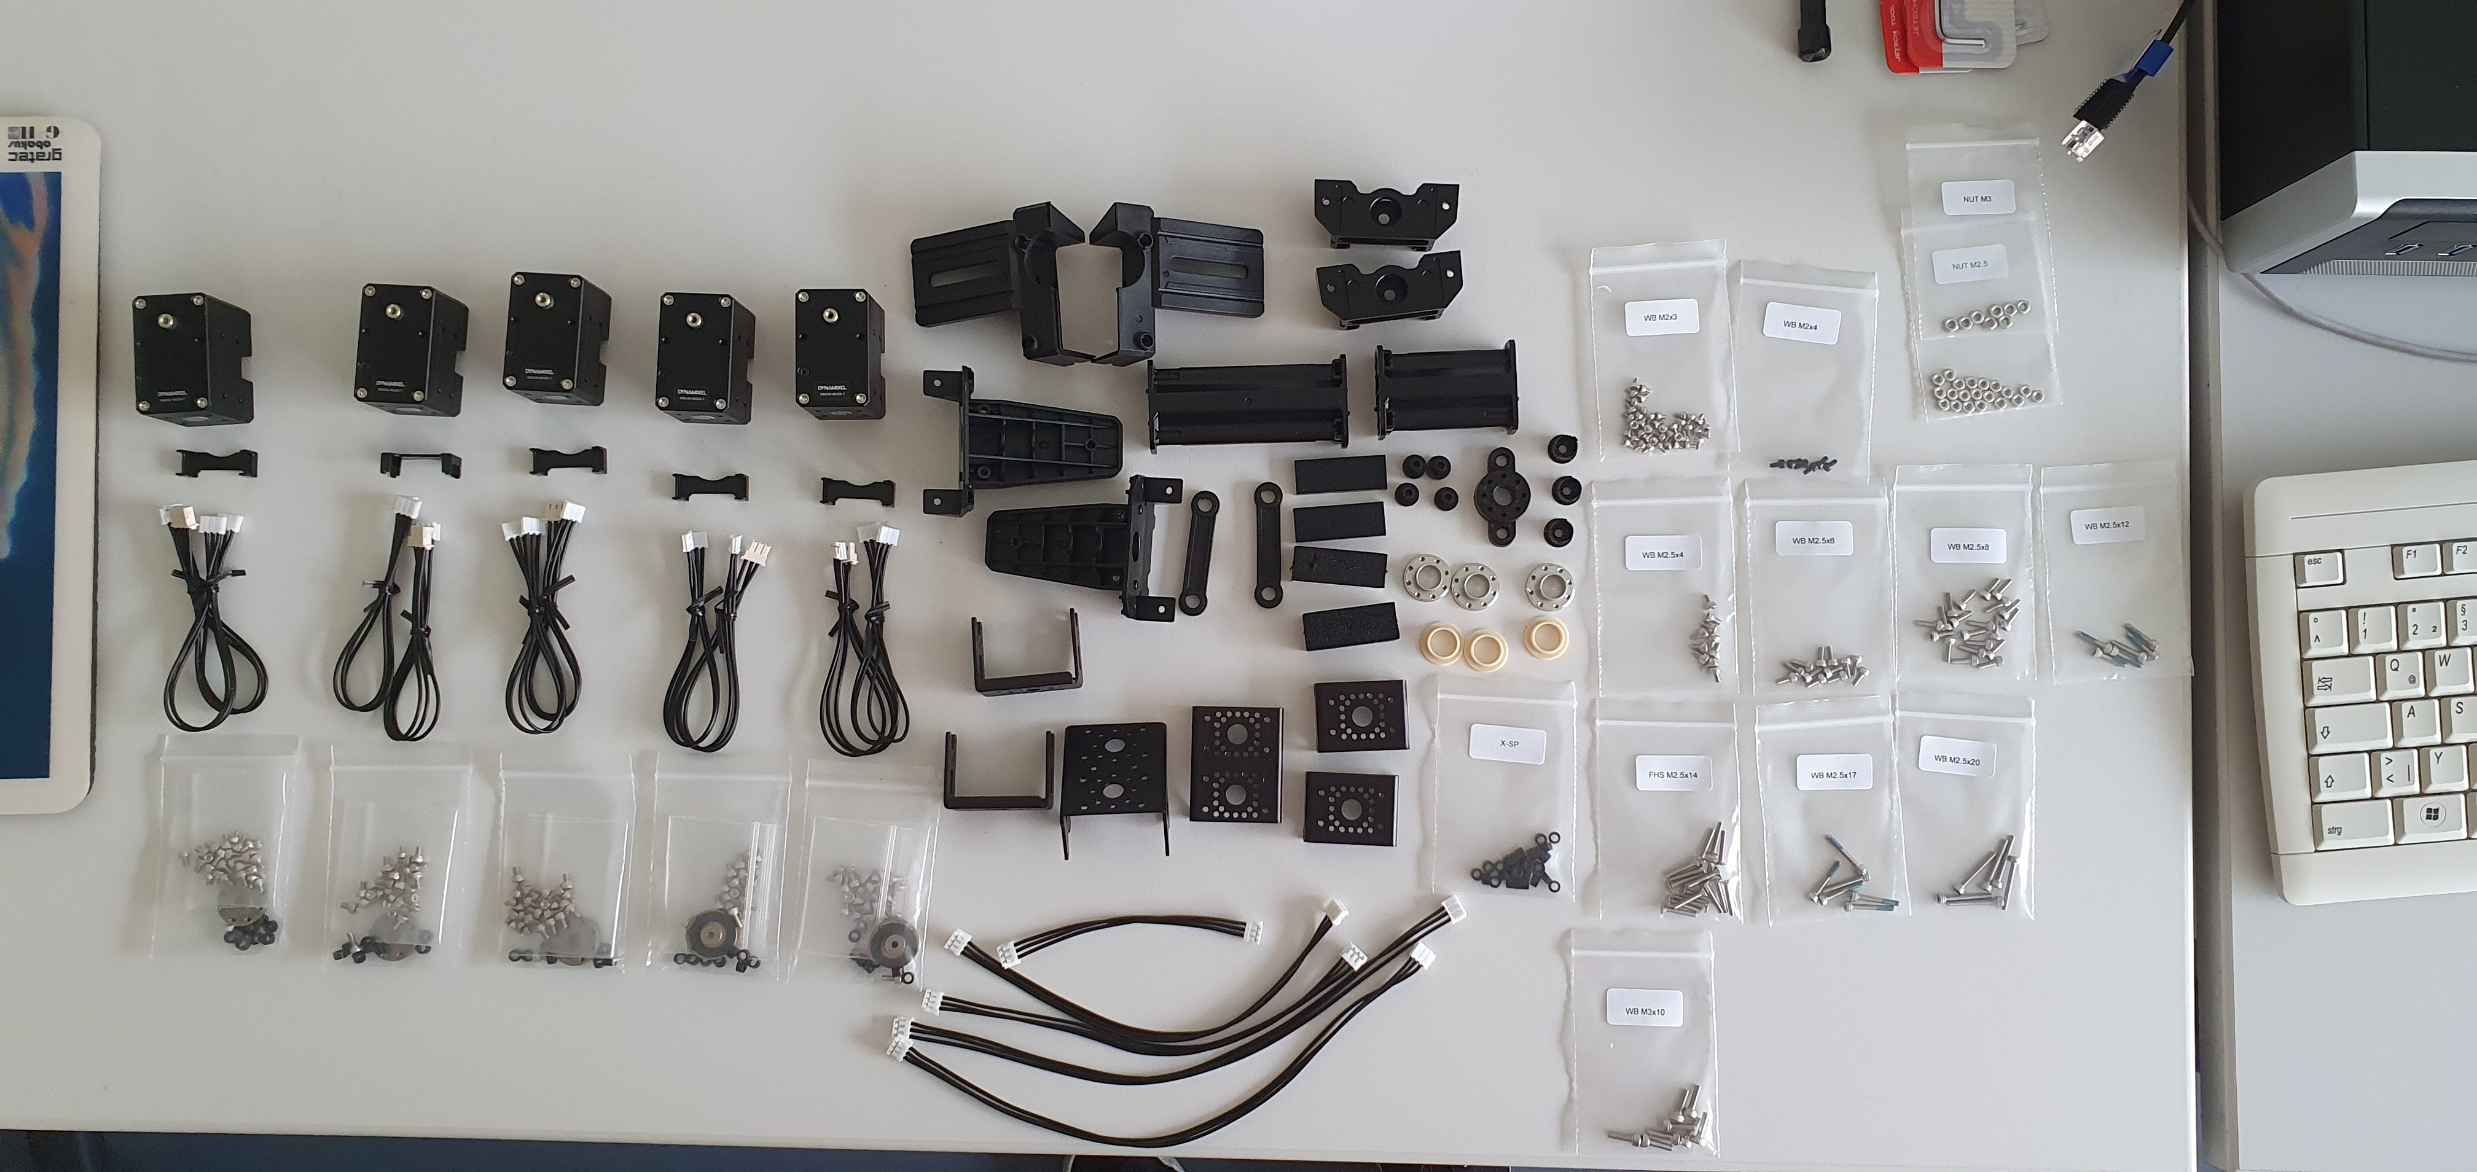
\includegraphics[width=\textwidth]{parts}
\caption{Bausatz für den OpenMANIPULATOR-X}
\label{fig:omxparts}
\end{figure}
\subsubsection{Virtuelle Maschine}
Zur Nutzung des Greifarms wurde eine \ac{VM} mit VirtualBox {\footnote{https://www.virtualbox.org}} von Oracle aufgesetzt.
Als Betriebssystem der \ac{VM} wurde das für ROS2 Foxy empfohlene~\citep{foxyreq} Ubuntu 20.04 {\footnote{\url{https://releases.ubuntu.com/20.04/}}} gewählt.
Danach wurde entsprechend der Anleitung für den OpenMANIPULATOR-X~\citep{foxyinstall} zuerst ROS 2 Foxy über das Installations-Skript von ROBOTIS und im Anschluss die für den Greifarm benötigten Packages installiert.

\subsection{Steuerung OMX}
Die Steuerung des OMX erfolgt über die vom \emph{open\_manipulator\_x\_controller}\\ \verb|open_manipulator_x_controller| zur Verfügung gestellten Topics und Services.

\subsubsection{Anschluss über U2D2}{\label{u2d2}}
Der OMX wird über das U2D2 und das U2D2 Power Hub Board (s. Abbildung~\ref{fig:u2d2}) per USB an den PC angeschlossen.\\
Das U2D2 konvertiert die Signale der DYNAMIXEL und ermöglicht die Kontrolle über den PC.
Zur Nutzung des U2D2 in der \ac{VM} muss das Gerät \emph{FTDI USB <-> Serial Converter} über das Geräte-Menü der \ac{VM} an diese gebunden werden (s. Abbildung~\ref{fig:ftdivm}).
\begin{figure}[ht!]
\centering
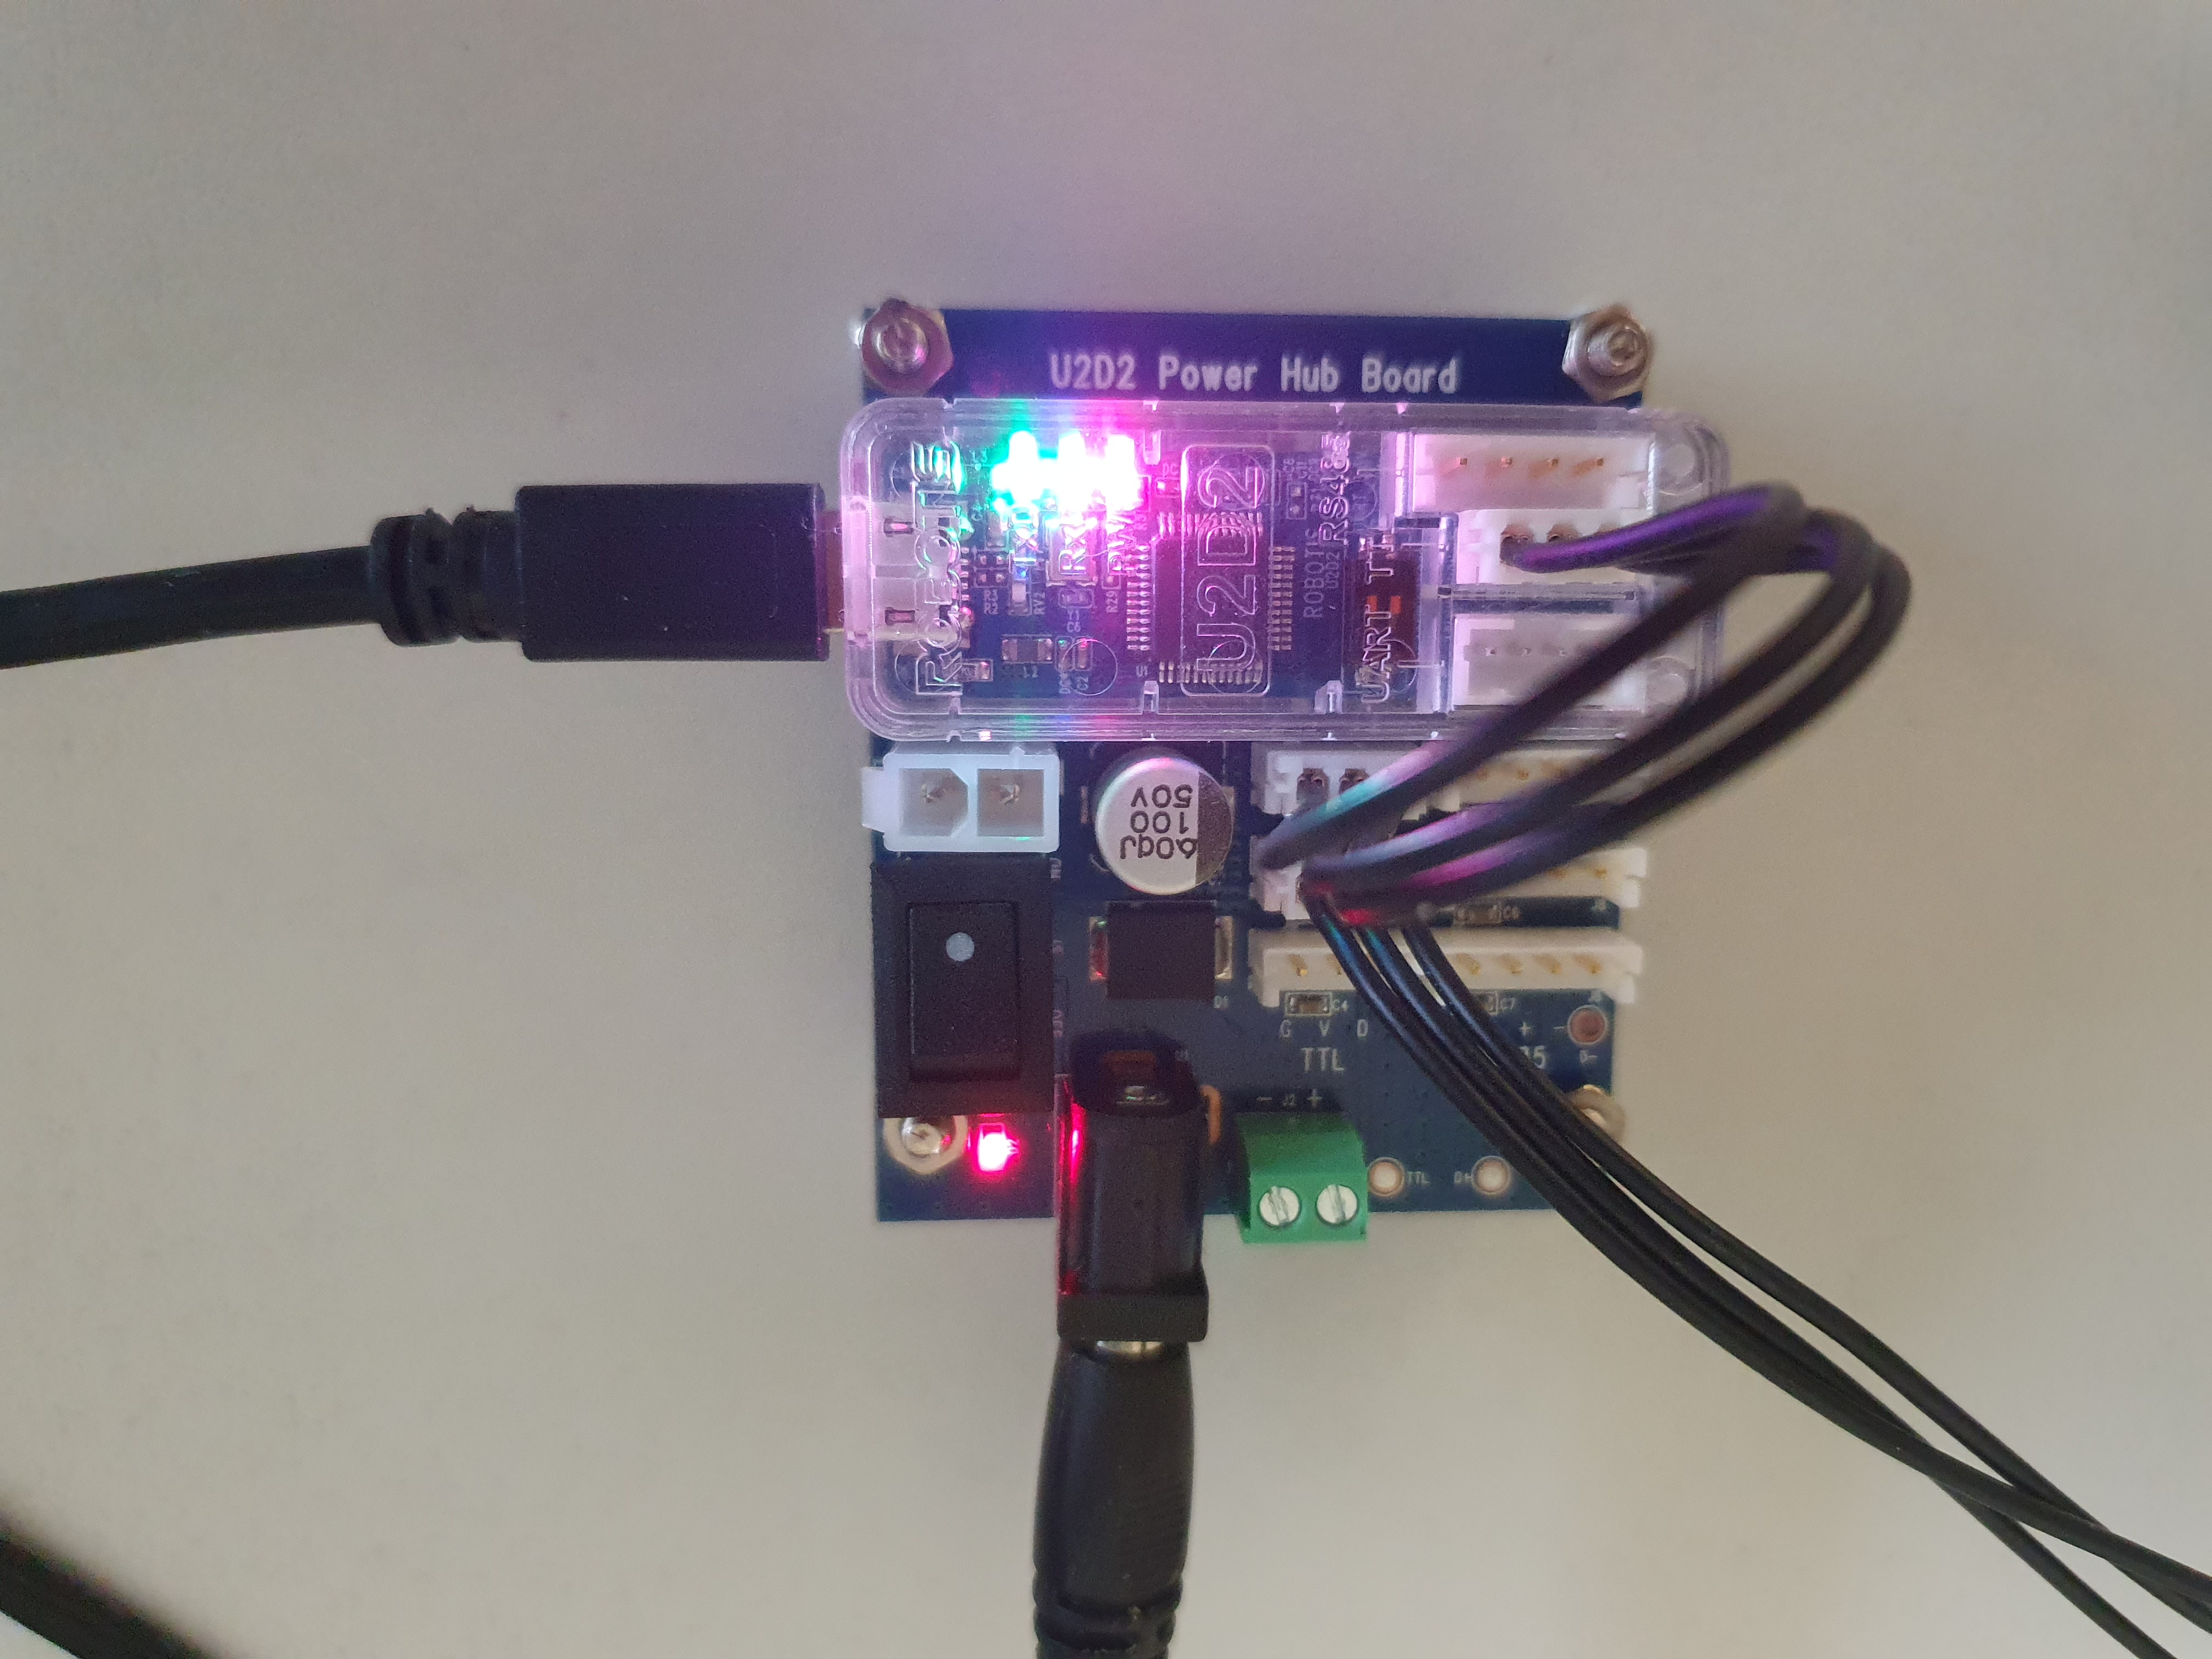
\includegraphics[width=\textwidth]{u2d2}
\caption{U2D2 Power Hub Board mit montiertem U2D2 (rechts im Bild)}
\label{fig:u2d2}
\end{figure}
\begin{figure}[ht!]
\centering

\includegraphics[width=\textwidth]{ftdivm}
\caption{Geräte-Menü der \ac{VM} mit angeschlossenem U2D2}
\label{fig:ftdivm}
\end{figure}


\subsubsection{OMX-Controller}
Der OMX-Controller ist ein Package, welches automatisch beim Installieren der für den OMX benötigten Software installiert wird.
Er kann über die entsprechende Launch-Datei mit dem Befehl
\begin{verbatim}
ros2 launch open_manipulator_x_controller 
     open_manipulator_x_controller.launch.py
\end{verbatim}
gestartet werden.\\
Für eine Nutzung des OMX ist dieses Package zwangsläufig nötig, da es alle Steuerungsmöglichkeiten sowie Informationen über den OMX zur Verfügung stellt.
\subsubsection{Joint und Task Space}
Der OMX kann in den zwei verschiedenen Arbeitsräumen \emph{Joint Space} und \emph{Task Space} betrachtet werden.\\
Im \emph{Joint Space} werden die Gelenke und ihre aktuellen Winkel betrachtet.\\
Der \emph{Task Space} entspricht einer Betrachtung in einem kartesischen Koordinatensystem, mit dem Motor mit der ID 11 als Ursprung.
Zusätzlich zur Position gibt es eine Orientierung für jede Achse (Roll-Nick-Gier, engl.\ roll-pitch-yaw).
\subsubsection{Topics}
Der OMX-Controller veröffentlicht drei Topics, die Informationen über den aktuellen Status geben:
\begin{itemize}
    \item /states
    \item /joint\_states
    \item /kinematics\_pose
\end{itemize}
\emph{/states} stellt allgemeine Informationen über die Motoren und die Bewegung des OMX zur Verfügung.
Ob die Motoren aktiviert sind, wird über das Feld \emph{open\_manipulator\_actuator\_state} mit den möglichen Werten \emph{ACTUATOR\_ENABLE} und \emph{ACTUATOR\_DISABLE} angegeben.
Der Bewegungsstatus, mit den möglichen Werten \emph{IS\_MOVING} und \emph{STOPPED}, steht im Feld \emph{open\_manipulator\_moving\_state}.\\
\emph{/joint\_states} stellt Informationen über alle Gelenke zur Verfügung.
Dies umfasst den Namen, den aktuell verbrauchten Strom, die Position (der Winkel des Motors) sowie die Geschwindigkeit.\\
\emph{/kinematics\_pose} stellt Informationen über die Pose im Task Space zur Verfügung.
Eine Pose besteht dabei aus einer Position und einer Orientierung und bezieht sich auf den Greifer.
Die Position enthält die Koordinaten der Mitte des Greifers.
Die Orientierung gibt die Rotation als Quaternion an.

\subsubsection{Kinematik}
Der OMX lässt sich über zwei Formen der Kinematik steuern.
Zum eine über die direkte Kinematik (auch Vorwärtskinematik, engl.\ forward kinematics, FK), was einer Steuerung im Joint Space entspricht und zum anderen über die inverse Kinematik (engl.\ inverse kinematics, IK), was einer Steuerung im Task Space entspricht.\\
Die komplette kinematische Steuerung erfolgt über Services, die sich dementsprechend darin unterscheiden, ob Winkel für die Gelenke oder Posen für den Greifer angegeben werden.
Bei der Steuerung über Posen besteht wiederum die Möglichkeit Position und Orientierung oder nur eines der beiden zu steuern und den aktuellen Wert des anderen beizubehalten.\\
Die komplette Liste der Services ist in der Anleitung des OMX\footnote{\url{https://emanual.robotis.com/docs/en/platform/openmanipulator_x/ros_controller_msg/#message-list}} zu finden.


\subsubsection{Teleop} \label{teleop}
Mit einem laufenden OMX-Controller kann der OMX auch ohne extra Programmierung direkt ferngesteuert werden.
Mögliche Geräte zur Steuerung sind die Tastatur sowie Playstation- und XBOX-Controller.
Für \ac{ROS2} Foxy wird aktuell allerdings nur die Steuerung über die Tastatur unterstützt.\\
Der OMX kann dabei sowohl im Task Space als auch im Joint Space kontrolliert werden (s. Abbildung~\ref{fig:teleopkeyboard}).
Zusätzlich gibt es 2 vordefinierte Posen (Init und Home) in die der OMX bewegt werden kann (s. Abbildung~\ref{fig:teleopposes}).
\begin{figure}[ht!]
\centering
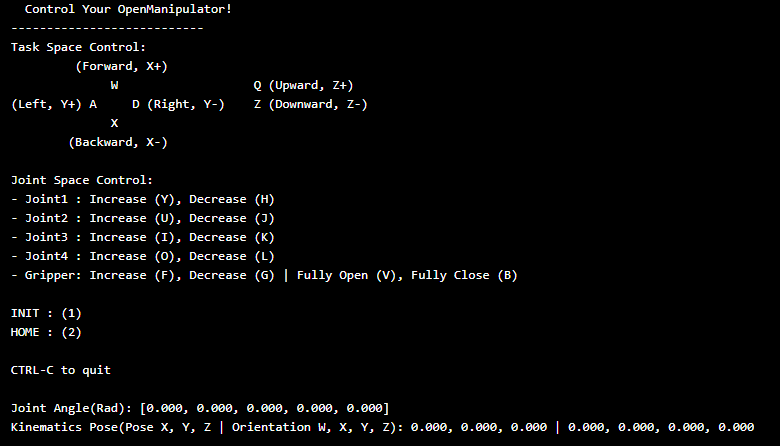
\includegraphics[width=\textwidth]{teleopkeyboard}
\caption{Fernsteuerung des OMX über die Tastatur}
\label{fig:teleopkeyboard}
\end{figure}
\begin{figure}[htb]
    \centering
    \begin{minipage}[t]{0.45\linewidth}
        \centering
        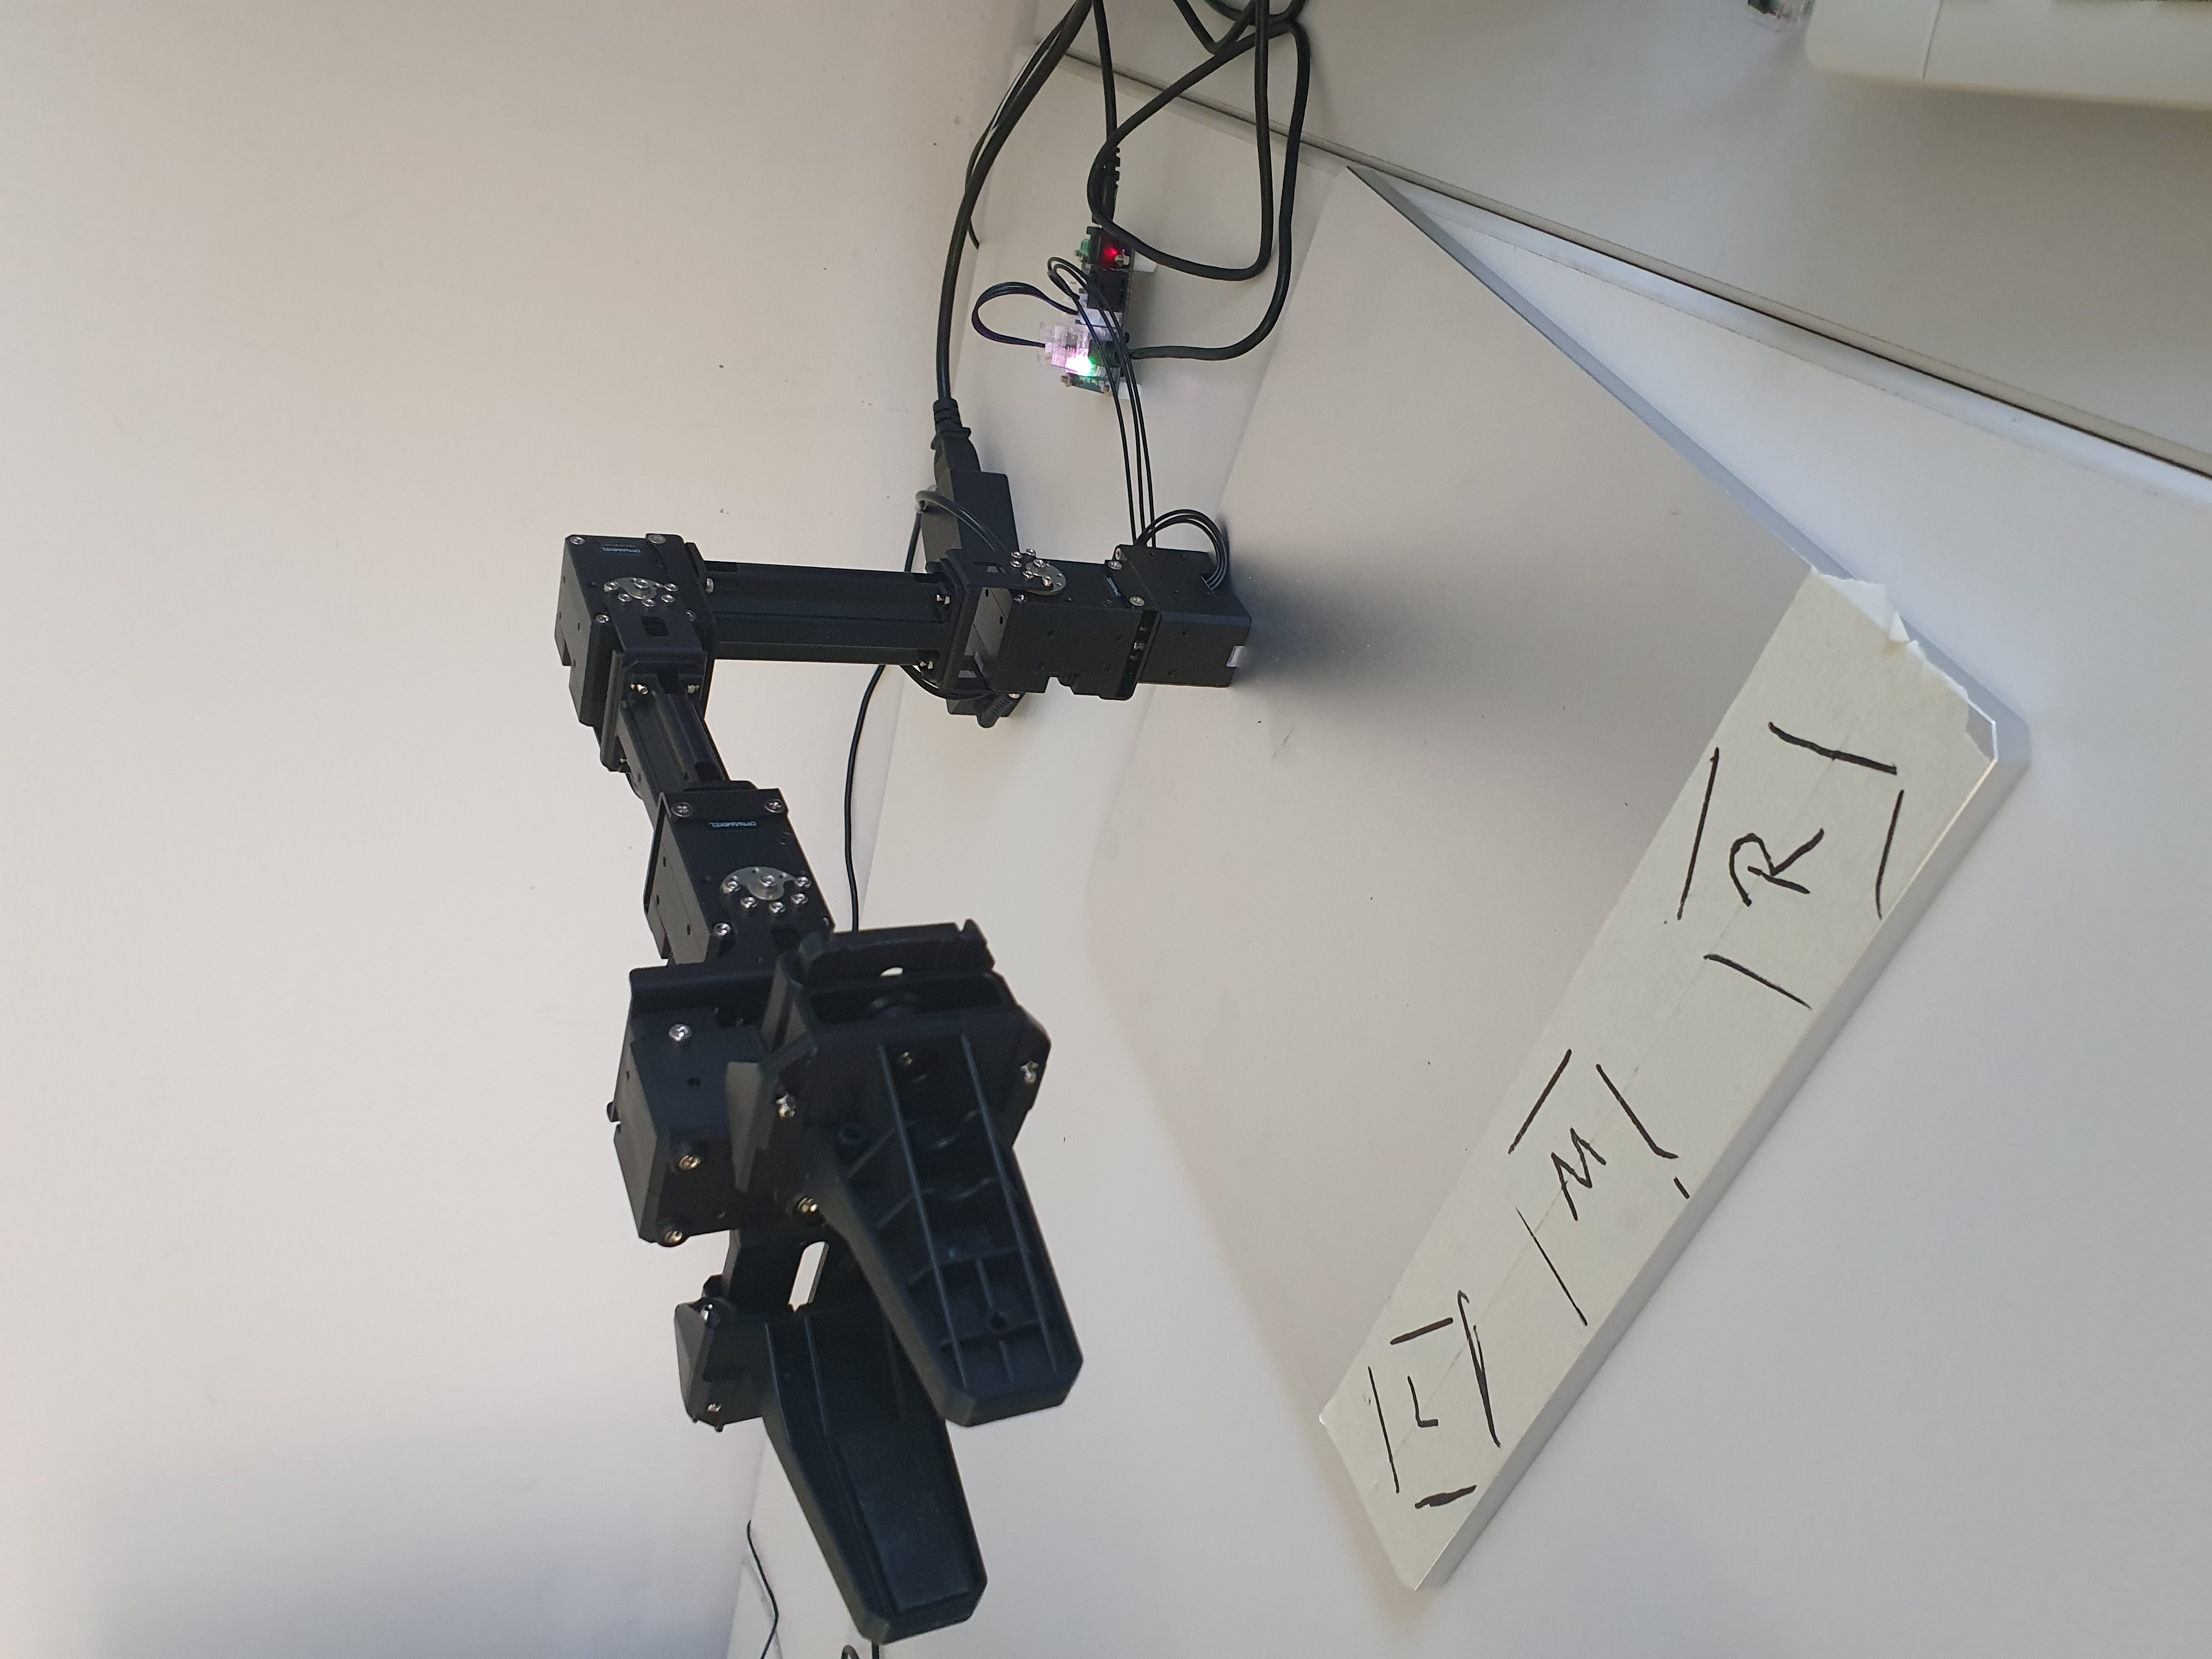
\includegraphics[width=\linewidth,keepaspectratio]{initpose}
    \end{minipage}% <- sonst wird hier ein Leerzeichen eingefügt
    \hfill
    \begin{minipage}[t]{0.45\linewidth}
        \centering
        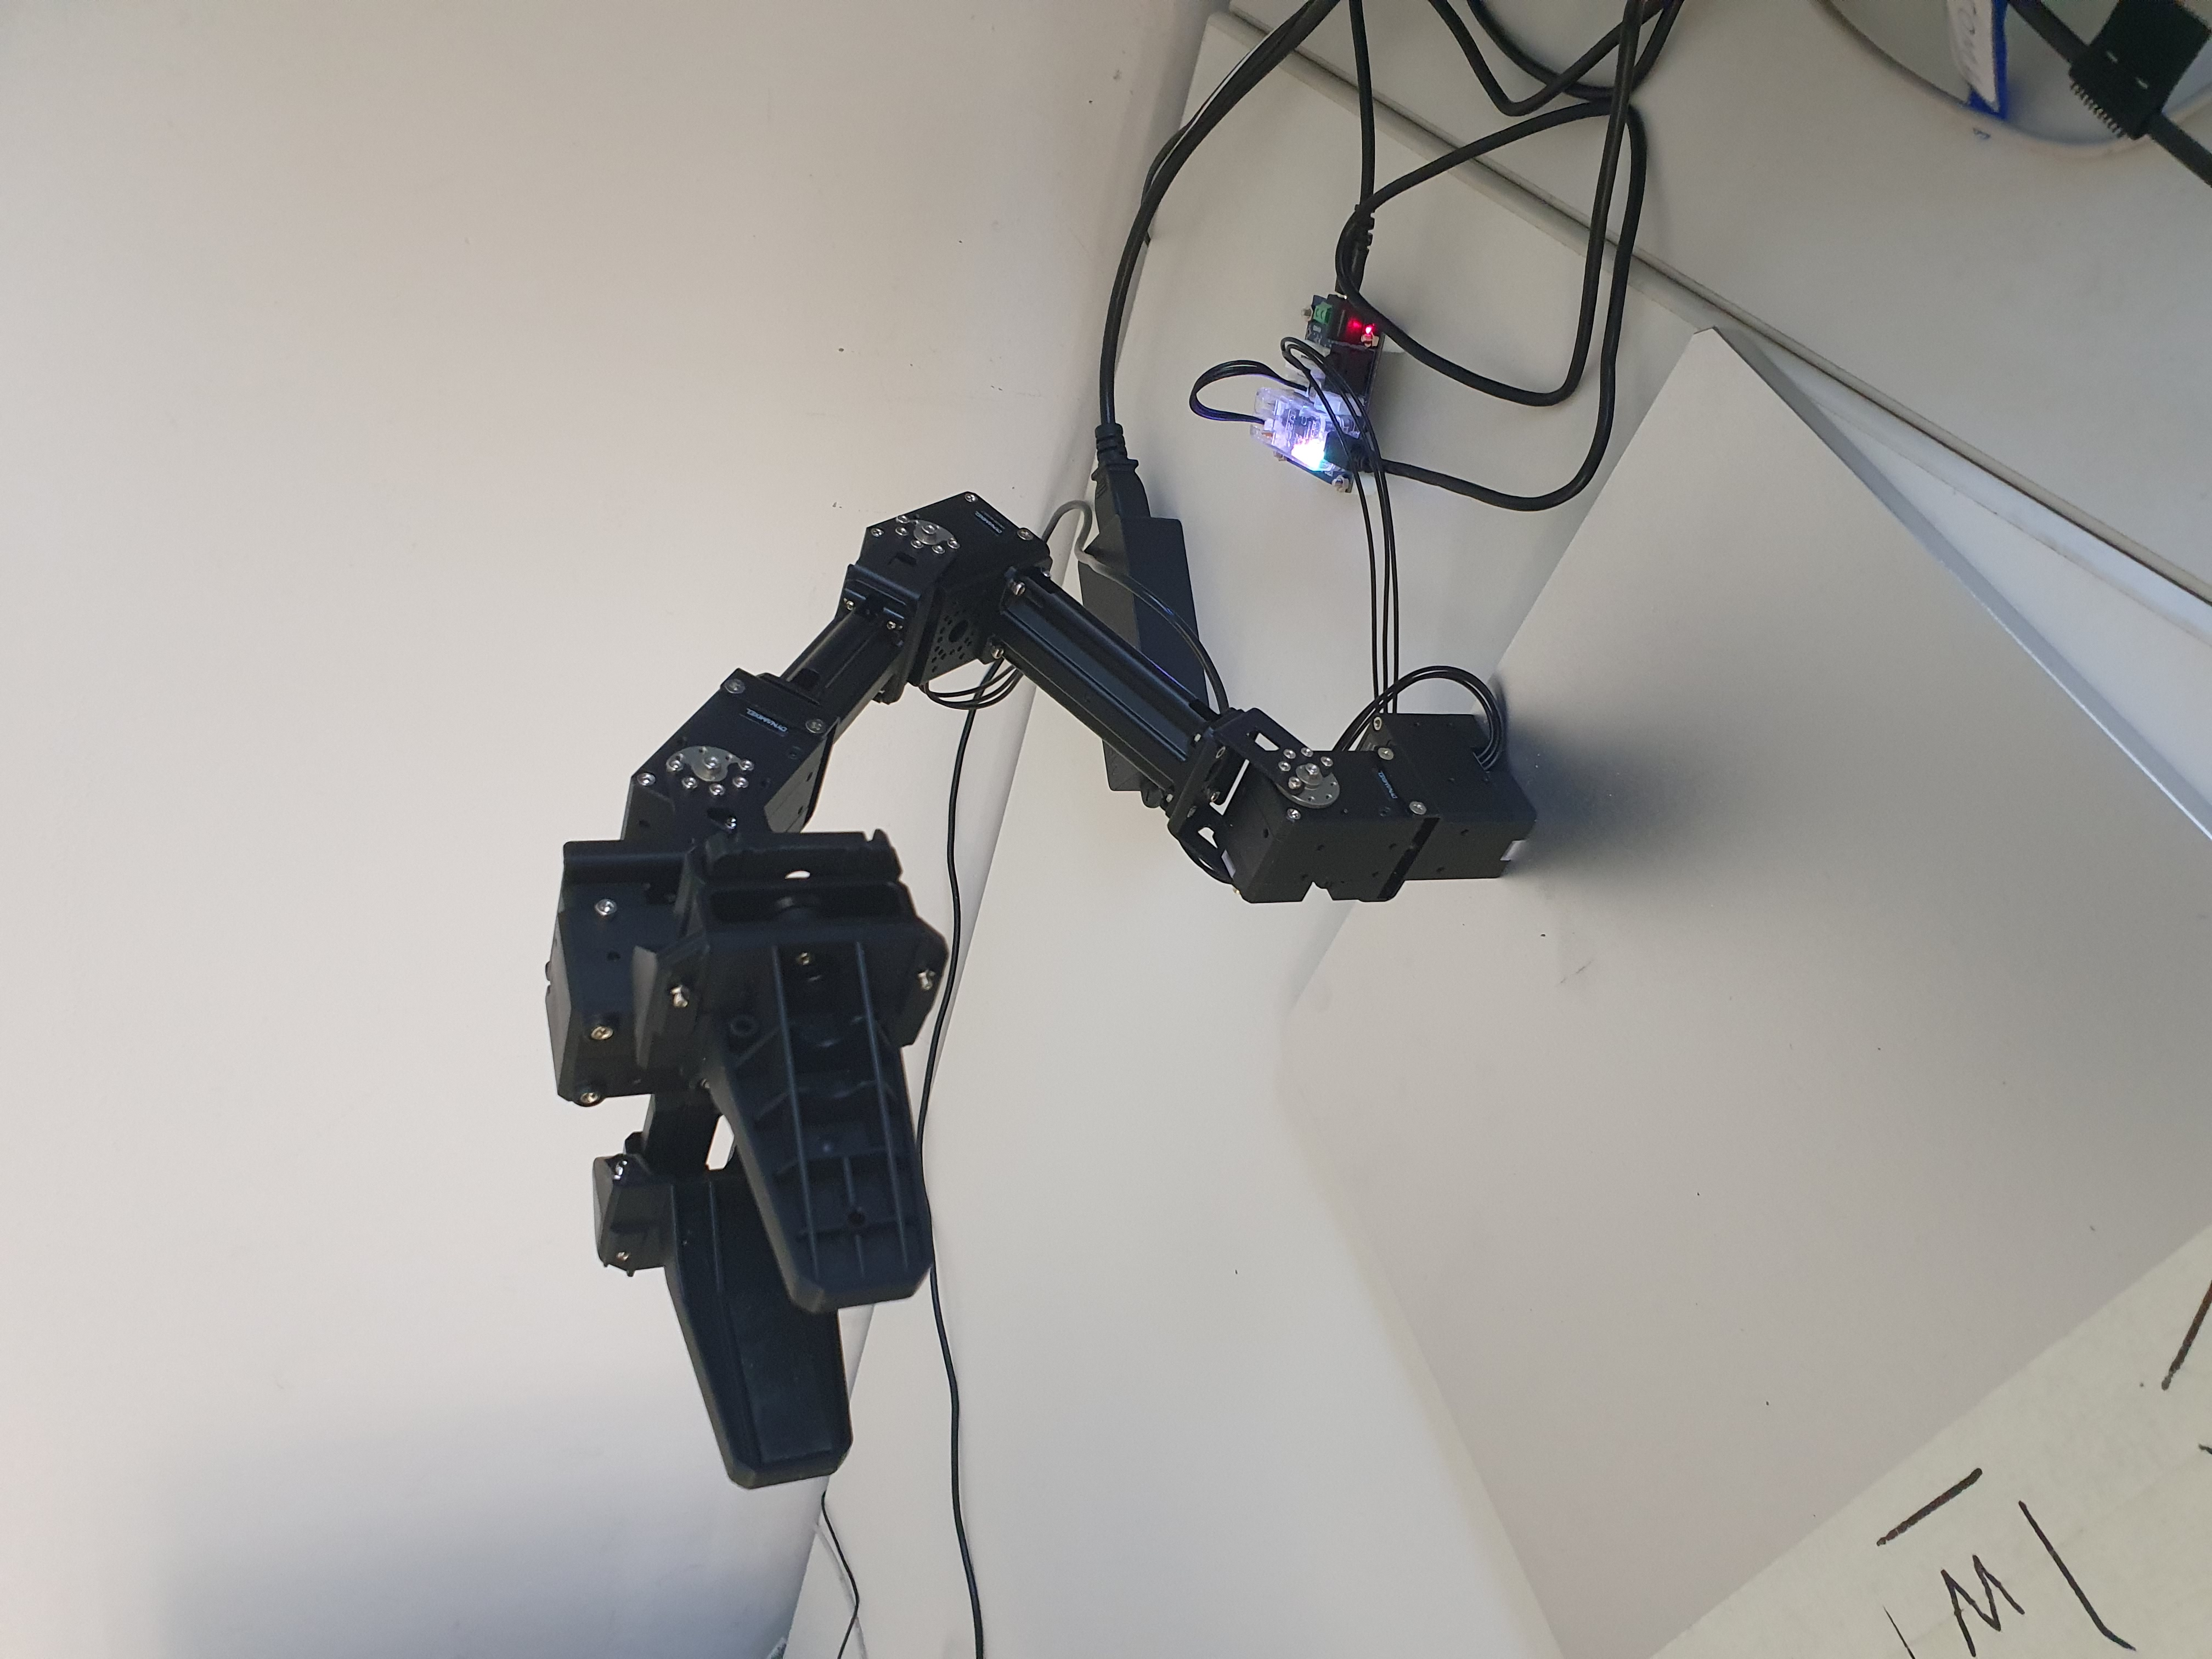
\includegraphics[width=\linewidth,keepaspectratio]{homepose}
    \end{minipage}
    \caption{Init (l.) und Home (r.) Pose der Tastatur Teleop}
    \label{fig:teleopposes}
\end{figure}



\subsection{PlanSys2}~\cite{plansys}\\
Für die Implementierung der in Abschnitt~\ref{konzept:nodes} genannten Funktionalitäten wird das Framework \ac{PlanSys2} genutzt.
Es übernimmt dabei alle Funktionalitäten: die Verwaltung der Daten zur Domäne und dem aktuellen Problem erfolgt über die domain-expert und problem-expert Nodes.
Die planer Node ist für die komplette Planung zuständig und die Executioner Node für die Ausführung des Plans.\\
Es müssen hier lediglich die Domäne erstellt sowie die tatsächliche Funktionalität der einzelnen Aktionen implementiert werden.
Das Wort Action im Namen der Nodes und den folgenden Kapiteln bezieht sich hier auf die Aktionen der Domäne, nicht auf \ac{ROS2} Actions.



\subsubsection{PDDL-Domain}
Beim erstellen der Domäne ist zu beachten, das \ac{POPF} nicht alle Funktionen unterstützt, die mit PDDL beschrieben werden können.
Dies beinhaltet unter anderem existentielle sowie negative Vorbedingungen.
Die vollständige Liste ist auf~\ref{popfpddlsupport} zu finden.\\
Für den Blockworld Teil der Domäne gibt es zunächst den Typ \verb|box| und Prädikate, die das Stapeln von Blöcken darstellen.
Dies umfasst das Verhältnis von Blöcken aufeinander (\verb|(box_on ?b_above ?b_below - box)|) sowie ob ein Block der oberste eines Stapels und damit frei zum bewegen ist (\verb|(clear ?b - box)|).
Als Aktionen werden das Nehmen sowie Ablegen eines Blocks benötigt.
Da in den Bedingungen und Effekten einer Aktion nur mit Parametern gearbeitet werden kann, welche auch Parameter der Aktion selbst sind, wird hier weiter aufgeteilt in Nehmen/Ablegen eines Blocks von/auf einen anderen Block sowie von/auf einen leeren Stapel.
Für das Bewegen von Blöcken ergeben sich die 4 Aktionen \verb|GRAB, PLACE, STACK, UNSTACK|.\\
Während für das reine Stapeln der Blöcke die exakte Position dieser nicht wichtig ist, wird diese jedoch für den Greifer benötigt, welcher vor diesen Aktionen an die richtige Stelle bewegt werden muss.
Hier werden die weiteren Typen \verb|location| und \verb|stack| sowie die Prädikate \verb|(box_at ?b - box ?l - location)|,\\ \verb|(gripper_at ?g - gripper ?l - location)|,\\ \verb|(location_above ?l_above ?l_below - location)| und\\ \verb|(is_base_loc ?l - location ?s - stack)| eingeführt.\\ \\
Das Prädikat \verb|clear| ist notwendig, da \ac{POPF} weder existentielle noch negative Vorbedingungen unterstützt.
Es wird genutzt um zu überprüfen, ob ein Block der oberste eines Stapels ist, was es ermöglicht diesen zu nehmen oder einen anderen auf diesem abzulegen.
Durch existentielle und negative Vorbedingungen könnte dies für die Aktion den Block B zu greifen, durch eine Bedingung der Form ''es existiert kein Block C für den gilt:( box\_on C B)'' ersetzt werden. \\ \\
Da alle Aktionen eine Dauer haben und \ac{PlanSys2} auch nur diese unterstützt, werden alle Aktionen als \verb|durative-action| modelliert.
Es wird jeder Aktion eine Dauer zugeordnet (\verb|:duration (= ?duration 0.25)|) welche auch für Metriken genutzt werden kann.
Zusätzlich bekommen Bedingungen und Effekte einen temporalen Zusatz: \verb|at start| und \verb|at end| können sowohl für Bedingungen als auch Effekte benutzt werden, um festzulegen zu welchem Zeitpunkt der Aktion diese Bedingung zutreffen oder der Effekt eintritt.
Für Bedingungen gibt es außerdem \verb|over all| damit eine Bedingung über die komplette Dauer der Aktion zutreffen muss damit sie gültig ist.\\
Da Bedingungen dadurch nicht mehr strikt vor Ausführung der Aktion gelten müssen, wird das Schlüsselwort \verb|:precondition| zu \verb|:condition| geändert.
Im aktuellen Szenario wird \verb|over all| dafür genutzt, allen Block-Aktionen die Bedingung zu geben, dass sich der Greifer über die komplette Zeit an der gleichen Stelle wie der entsprechende Block befinden muss.\\
Nur in der \verb|MOVE-GRIPPER| Aktion wird \verb|at start| für einen Effekt genutzt:\\
\verb|(at start(not (gripper_at ?g ?l_from)))|.\\
Sobald die Aktion beginnt befindet sich der Greifer nicht mehr an der Ausgangsposition und erst am Ende der Aktion wird die neue Position als Fakt gesetzt:\\
\verb| (at end(gripper_at ?g ?l_to))|.
Würden beide Effekte erst am Ende der Aktion eintreten, würde der Planer mehrere \verb|MOVE-GRIPPER| Aktionen parallel ausführen (s. Abbildung~\ref{fig:tempgrippereffect}).
Dies ist zum einen physisch nicht möglich, hinterlässt die Welt aber auch in einem ungültigen Zustand, da der Greifer sich dann an mehreren Positionen gleichzeitig befinden würde.

\subsubsection{Action Nodes}
Obwohl in der Domäne mehr als 2 Aktionen beschrieben sind, beschränken sich die ausgeführten Aktionen auf ein Bewegen des OMX sowie die Kontrolle des Greifers.
Für diese wird jeweils eine Node erstellt.
Damit diese Nodes von \ac{PlanSys2} genutzt werden können, müssen sie von der Basisklasse \verb|plansys2::ActionExecutorClient| erben.
Da diese von \ac{PlanSys2} nur in C++ zur Verfügung gestellt wird, müssen auch die Aktionen in C++ implementiert werden.\\
In jeder Aktion muss die Methode \verb|void do_work()| implementiert werden.
Diese wird mit einem bestimmten Zeitintervall aufgerufen während die Aktion aktiv ist.
Das Intervall wird im Konstruktor gesetzt (s. Zeile~\ref{code:line:nodeintervall} in~\ref{code:gripperactionnode}).
Das Mapping einer Node zu einer Aktion erfolgt durch das Setzen des Parameters \verb|action_name| nach dem Erstellen der Node (s. Zeile~\ref{code:line:actionname} in~\ref{code:gripperactionnode}).

\subsubsection{Control Gripper Aktion}
Die Logik Node zur Steuerung des Greifers wird in der Klasse \verb|ControlGripperAction| (s.~\ref{code:gripperactionnode}) implementiert.
Da es vom OMX kein Feedback gibt, ob oder wann etwas gegriffen wurde, wird die Aktion mit einer fixen Wartezeit implementiert: wenn die Aktion gestartet wird, wird ein Request zur Steuerung des Greifers erzeugt (s. Zeile~\ref{code:line:gripperrequest} in~\ref{code:gripperactionnode}) und gesendet und nach einer bestimmten Zeit die Aktion beendet.
Um unnötige Aufrufe der Methode während des Wartens zu verhindern wird die Wartezeit über das Zeitintervall zur Ausführung der Node gesetzt.
Die Aktion wird hierdurch immer beim 2.\ Aufruf der Methode \verb|do_work| beendet.\\
Zum Senden des Requests wird ein \ac{ROS2} Client für den Service \verb|goal_tool_control| mit dem Typ \verb|open_manipulator_msgs::srv::SetJointPosition| erstellt. 
Um sowohl die Aktionen zum Öffnen sowie Schließen des Greifers mit einer Node implementieren zu können wird ein Parameter eingeführt, welcher über den Konstruktor gesetzt wird und die Bewegung des Greifers bestimmt.
Für jede Aktion wird eine Node mit entsprechenden Parametern erzeugt.
Diese Nodes werden alle einem \verb|MultiThreadedExecutor| hinzugefügt. Dadurch können alle Nodes gemeinsam gestartet werden und laufen in einem Prozess, sind durch mehrere Threads aber unabhängig voneinander.

\subsubsection{Move Gripper Aktion}
Die Logik Node zur Bewegung des OMX wird in der Klasse \verb|MoveGripperAction| (s.~\ref{code:moveactionnode}) implementiert.
Insgesamt umfasst dies das Senden des Bewegungsrequests an den vom OMX-Controller erstellten Service \verb|goal_task_space_path_position_only| mit dem Typ \verb|open_manipulator_msgs::srv::SetKinematicsPose| (s. Zeile~\ref{code:line:poseclient} in\ref{code:moveactionnode}) sowie das Beenden der Aktion wenn der OMX an der Zielposition angekommen ist.
Ob die Bewegung beendet ist wird über den im Topic \verb|states| gesendeten Bewegungsstatus geprüft.
Dieser kann die beiden Werte \verb|IS_MOVING| und \verb|STOPPED| annehmen.
Der aktuelle Status wird mit dem letzten empfangenen verglichen: war der letze Status \verb|IS_MOVING| und der aktuelle \verb|STOPPED|, waren wir in einer Bewegung, die jetzt beendet ist.\\
Um die Zielkoordinaten der Bewegung zu erhalten, muss der String Parameter der Aktion in Zahlenwerte konvertiert werden.
Zunächst werden aus dem String, welcher im Format \verb|s<Nummer des Stapels>l<Höhe innerhalb eines Stapels>| vorliegt, die 2 Integerwerten mit Hilfe einer regular Expression extrahiert.
Diese werden im 2.\ Schritt über Maps zu Y und Z Koordinaten konvertiert.
Die X Koordinate ist im Rahmen dieser Arbeit fest auf den Wert 0,25 gesetzt.\\
Um eine kollisionsfreie Bewegung sicherzustellen findet diese nicht direkt von der aktuellen zur Zielposition statt.
Stattdessen werden mehrere Zwischenpositionen errechnet und entsprechende Bewegungen zuerst ausgeführt.
Zunächst wird der OMX bei gleichbleibenden X und Y Koordinaten auf eine Z Koordinate von 0,25 bewegt.
Dies entspricht eine Höhe in der keine Blöcke liegen können.
Die zweite Zwischenposition bleibt auf der gleichen Höhe (Z Koordinate 0,25) und bewegt sich zur X und Y Koordinate der Zielposition.
Diese Zwischenposition befindet sich exakt oberhalb der Zielposition, sodass eine vertikale Bewegung zur Zielposition ohne Kollision möglich ist.\\
Diese Zwischenpositionen werden übersprungen, wenn die aktuelle Position des OMX bereits dem korrekten Stapel der Zielposition entspricht.
Hierbei werden die aktuellen Koordinaten auf 2 Dezimalstellen gerundet.\\
Für alle benötigten Positionen wird ein Request erzeugt und einer Queue hinzugefügt.
Der Auslöser, den nächsten Request zu senden ist jeweils das Ende der vorherigen Bewegung.\\
Um Zugriff auf die aktuelle Position des OMX zu erhalten wird ein weiterer Subscriber für das Topic \verb|kinematics_pose| benötigt, welches eine Message vom Typ\\
\verb|open_manipulator_msgs::msg::KinematicsPose| veröffentlicht.\\
Um eine Beschädigung der Motoren zu vermeiden, soll die Bewegung bei einer Kollision abgebrochen werden.
Hierfür sind zwei Teile nötig: die Kollisionserkennung sowie das Abbrechen der Bewegung.
Für die Kollisionserkennung wird der Stromverbrauch der einzelnen Motoren genutzt.
Dieser steigt, wenn der Motor mehr Leistung bringen muss, wenn versucht wird sich gegen ein Hindernis zu bewegen.\\
Dieser ist in der Message des Topics \emph{joint\_states} als \emph{effort} enthalten.
Die letzten $x$ Werte (konfigurierbar über die Variable \emph{EFFORT\_COUNT}, standardmäßig 10) werden für jeden Motor gespeichert (s. Zeile~\ref{code:line:effortsaving} in \ref{code:moveaction}) und ausgewertet (s. Zeile~\ref{code:line:efforteval} in \ref{code:moveaction}).
Die Werte jedes Motors werden einzeln ausgewertet.
Es wird das Maximum und das Minimum der Werte genommen und geprüft ob die absolute Differenz größer als der festgelegte Grenzwert (konfigurierbar über die Variable \emph{EFFORT\_THRESHOLD}, standardmäßig 500) ist.
Ist dies für mindestens einen Motor der Fall gilt die Aktion als fehlgeschlagen und der entsprechende Status wird zurückgegeben (s. Zeile~\ref{code:line:effortfail} in \ref{code:moveaction}).
Eine fehlgeschlagene Aktion resultiert gleichzeitig in einem fehlgeschlagenen Plan.
Ein Abbrechen der Aktion verhindert jedoch nicht, dass der OMX versucht das aktuelle Bewegungsziel zu erreichen.
Es wird ein neues Bewegungsziel erstellt, das sich an der aktuellen Position befindet.


\subsubsection{Package}
- pkg build config\\
Alle erstellten Komponenten werden in einem eigenen \ac{ROS2} Package gebündelt.
Dies umfasst die C++ Dateien für die Aktionen sowie die Domänendatei.
Es wurde eine Launch Datei erstellt um das komplette System über einen Befehl starten zu können.
In der Launch Datei wird zum einen \ac{PlanSys2} und zum anderen die Nodes für alle Aktionen gestartet.
Weiterhin wird hier festgelegt, welche Domäne genutzt wird.\\
Das Package enthält außerdem eine Readme Datei in der die nötigen Schritte beschrieben sind um das gesamte System, einschließlich OMX, zu starten.
Weiterhin wurden mehrere Problemszenarien erstellt, die sowohl als \ac{PDDL} Datei als auch als Befehle für das \ac{PlanSys2} Terminal zur Verfügung stehen.

\subsection{Praktische Anwendung}
Um das System praktisch anwenden zu können wurden mehrere farbige Würfel aus LEGO gebaut (s. Abbildung~\ref{fig:legocubes}).
Auf der Basisplatte des OMX wurden die Positionen für drei Stapel markiert.
Es werden mehrere Szenarien getestet um die allgemeine Anwendbarkeit zu überprüfen.
\subsubsection{PlanSys2 Terminal}
Das \ac{PlanSys2} Terminal ist eine separate Node, welche es ermöglicht, das System durch Eingabe über die Konsole zu steuern.
Die wichtigsten Befehle sind hierbei \verb|get|, \verb|set| und \verb|run|.
Mit \verb|get| können die Typen, Prädikate und Aktionen der geladenen Domäne sowie des aktuellen Problems angezeigt werden (s. Abbildung~\ref{fig:plansysterminal}).
Der \verb|set| Befehl wird genutzt, um das aktuelle Problem zu verändern.
Es können Instanzen, Prädikate sowie das Ziel erstellt und geändert werden.
Über den Befehl \verb|run| lässt sich der Plan für das aktuelle Ziel ausführen.
Es ist auch möglich nur einen Plan zu suchen, ohne ihn direkt auszuführen.
Dies ist mit \verb|get plan| möglich (s. Abbildung~\ref{fig:terminalplan}).\\
Während der Ausführung eines Plans wird im Terminal die aktuelle Aktion sowie dessen Fortschritt (gesteuert über den Feedback Kanal innerhalb der Aktion) angezeigt.
\subsubsection{Sussman Anomalie}
Die Sussman Anomalie~\cite{sussman} beschreibt eine Schwäche von Planern, bei der bereits ausgeführte Teile bzw. erreichte Unterziele rückgängig gemacht werden müssen um andere bzw. das Gesamtziel zu erreichen.
Dieses Problem kann durch drei Blöcke beschrieben werden, die sich Anfangs in den Positionen befinden, die in Abbildung~\ref{fig:sussmaninitial} gezeigt wird.
Das Ziel ist es, dass $A$ auf $B$ und $B$ auf $C$ gestapelt wird, wobei jeweils immer nur ein Block gewegt werden kann.
Wird versucht als erstes $A$ auf $B$ zu erfüllen, wird $C$ zur Seite gelegt und $A$ auf $B$ platziert (s. Abbildung~\ref{fig:sussmanab}).
Dieser Schritt muss nun wieder rückgängig gemacht werden um $B$ auf $C$ zu platzieren.\\
Wird stattdessen versucht als erstes $B$ auf $C$ zu erfüllen, so kann dies direkt durch bewegen von $B$ erreicht werden (s. Abbildung~\ref{fig:sussmanbc}).
Um das Ziel $A$ auf $B$ zu erfüllen muss dieser Schritt nun wieder rückgängig gemacht werden.
\begin{figure}[!htb]
    \minipage{0.32\textwidth}
    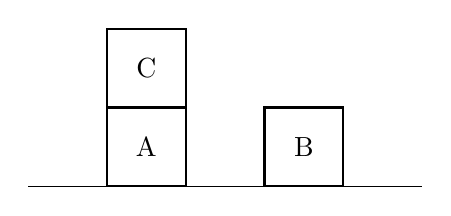
\begin{tikzpicture}
        \draw (-1,0) -- (4,0);
        \draw[black, thick] (0,0) rectangle (1,1) node[pos=.5] {A};
        \draw[black, thick] (0,1) rectangle (1,2) node[pos=.5] {C};
        \draw[black, thick] (2,0) rectangle (3,1) node[pos=.5] {B};
    \end{tikzpicture}
    \caption{Startzustand der Sussman Anomalie}\label{fig:sussmaninitial}
    \endminipage\hfill
    \minipage{0.32\textwidth}
    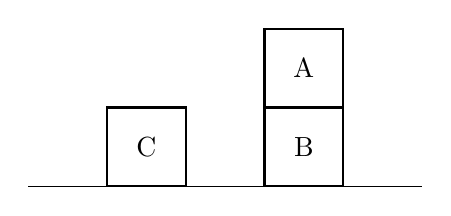
\begin{tikzpicture}
        \draw (-1,0) -- (4,0);
        \draw[black, thick] (0,0) rectangle (1,1) node[pos=.5] {C};
        \draw[black, thick] (2,1) rectangle (3,2) node[pos=.5] {A};
        \draw[black, thick] (2,0) rectangle (3,1) node[pos=.5] {B};
    \end{tikzpicture}
    \caption{Lösung des Teilziels $A$ auf $B$}\label{fig:sussmanab}
    \endminipage\hfill
    \minipage{0.32\textwidth}%
    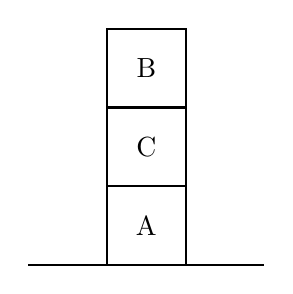
\begin{tikzpicture}
        \draw (-1,0) -- (2,0);
        \draw[black, thick] (0,0) rectangle (1,1) node[pos=.5] {A};
        \draw[black, thick] (0,1) rectangle (1,2) node[pos=.5] {C};
        \draw[black, thick] (0,2) rectangle (1,3) node[pos=.5] {B};
    \end{tikzpicture}
    \caption{Lösung des Teilziels $B$ auf $C$}\label{fig:sussmanbc}
    \endminipage
\end{figure}\\
Um diese Anomalie zu handhaben müssen Planer beide Ziele und deren Schritte kombinieren.
\ac{POPF} generiert für dieses Ziel den in Abbildung~\ref{fig:sussmanpopf} gezeigten Plan, der in Abbildung~\ref{fig:sussmanpopfvis} visualisiert wird.
Der grün hervorgehobene Block ist jeweils der, der in diesem Schritt bewegt wurde.
\begin{figure}[!htb]
    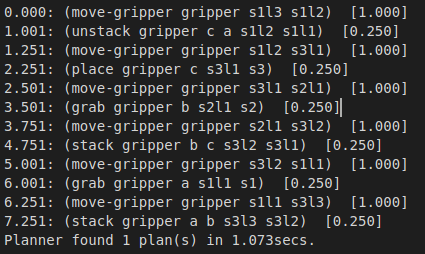
\includegraphics{sussmanpopfplan}
    \caption{Durch \ac{POPF} generierter Plan für die Sussman Anomalie}
    \label{fig:sussmanpopf}
\end{figure}
\begin{figure}[!htb]
    \begin{tikzpicture}
        \begin{scope}
            \draw (-0.5,0) -- (3,0);
            \draw[black, thick] (0,0) rectangle (1,1) node[pos=.5] {A};
            \draw[black, thick] (0,1) rectangle (1,2) node[pos=.5] {C};
            \draw[black, thick] (1.5,0) rectangle (2.5,1) node[pos=.5] {B};
        \end{scope}
        \draw[green, thick, 3pt, ->] (2.75,0.5) -- (3.75,0.5);
        \begin{scope}[xshift=4cm]
            \draw (-0.5,0) -- (4.5,0);
            \draw[black, thick] (0,0) rectangle (1,1) node[pos=.5] {A};
            \draw[black, thick] (1.5,0) rectangle (2.5,1) node[pos=.5] {B};
            \filldraw[color=black, fill=green!10, thick] (3,0) rectangle (4,1) node[pos=.5] {C};
        \end{scope}
        \draw[green, thick, 3pt, ->] (8.25,0.5) -- (9.25,0.5);
        \begin{scope}[xshift=9.5cm]
            \draw (-0.5,0) -- (3,0);
            \draw[black, thick] (0,0) rectangle (1,1) node[pos=.5] {A};
            \filldraw[color=black, fill=green!10, thick] (1.5,1) rectangle (2.5,2) node[pos=.5] {B};
            \draw[black, thick] (1.5,0) rectangle (2.5,1) node[pos=.5] {C};
        \end{scope}
        \draw[green, thick, 3pt, ->] (12.25,0.5) -- (13.25,0.5);
        \begin{scope}[xshift=13.5cm]
            \draw (-0.5,0) -- (1.5,0);
            \draw[black, thick] (0,0) rectangle (1,1) node[pos=.5] {C};
            \draw[black, thick] (0,1) rectangle (1,2) node[pos=.5] {B};
            \filldraw[color=black, fill=green!10, thick] (0,2) rectangle (1,3) node[pos=.5] {A};
        \end{scope}
    \end{tikzpicture}
    \caption{Visualisierte Lösung der Sussman Anomalie durch \ac{POPF}}
    \label{fig:sussmanpopfvis}
\end{figure}
\subsubsection{Mehr Blöcke, mehr Positionen}
\newpage
- evtl sinnvolle Auswertung der maximalwerte inkl. graphen\\
Die Anzahl der möglichen Blöcke und Positionen soll ausgereizt werden.
Bei einem Szenario mit drei Stapeln mit jeweils drei Positionen kann ein maximum von 9 Blöcken platziert werden.
Dies verhindert jedoch das Bewegen von Blöcken, da die einzige freie Position zu der ein aufgenommener Block bewegt werden kann, seine Ursprungsposition ist.
Um mehr Blöcke verwenden zu können müssen also die Anzahl der Stapel und/oder die maximale Höhe der Stapel erweitert werden.\\
Für beide Varianten gibt es Einschränkungen, die zu beachten sind.
Für höhere Stapel ist der Bewegungsraum des OMX zu beachten.
Über dem äußeren Rand der Grundplatte beträgt die maximale Höhe ca 25cm.
Da sich der Greifarm mit einem gegriffenem Block frei oberhalb der Stapel bewegen können muss, muss die maximale Höhe eines Stapels unterhalb dieses Werts liegen.
Die exakte Maximalhöhe ist von der Größe der Blöcke abhängig.\\
Für weitere Stapel nehmen wir als Vorraussetzung, dass alle Stapel sich nebeneinander befinden sollen.
Stapel die sich hinter einem anderen befinden, können vom OMX nicht garantiert frei angesteuert werden.
Je näher sich die Stapel am OMX befinden, desto größer ist der Winkel zwischen ihnen.
Aufgrund der größe des Greifers muss der Abstand zwischen mehreren Stapeln umso größer sein, je näher sie sich am OMX befinden.
Stapel sollen sich daher am äußeren Rand der Grundplatte befinden.\\
Da sowohl ein erhöhen der Anzahl der Stapel als auch deren Höhe durch die Größe der Blöcke behindert wird, wurden kleinere Blöcke gebaut.
Dies ermöglicht bis zu 5 Stapel mit einer maximalen Höhe von 5 Blöcken.
Das theoretische Limit an Blöcken wird damit auf 25, bzw. 24 um Bewegungen zu ermöglichen, erhöht.\\
Bereits Tests mit Zielen, deren Plan aus nur wenigen Schritten besteht, zeigen, das dies den Suchraum so stark erweitert, dass Pläne nicht oder erst nach langer Zeit gefunden werden.
Ein Testfall mit 20 Blöcken und dem Ziel den obersten Block eines Stapels auf den eines anderen zu legen (optimale Planlänge: 4) führte dazu, dass der Planer ca 13 Minuten lief.
Obwohl laut Konsolenausgabe ein Plan gefunden wurde, wird dieser nicht ausgegeben (s. Abbildung~\ref{fig:longplan}).\\
\emph{Hier sollten jetzt evtl Graphen und eine Auswertung stehen}\\
Während bei den wenigen, größeren Blöcken eine Namensgebung entsprechend der Farbe ausreichend war, wurden die kleineren Blöcke durchnummeriert.
Das \ac{PlanSys2} Terminal erlaubt zwar die Erstellung von Objekten und Prädikaten, die diese nutzen, mit rein numerischen Namen, stürzt jedoch beim Versuch ein Ziel mit diesen zu erstellen ohne aussagekräftige Fehlermeldung ab.
Ein weiteres Problem, das sich bei der Nutzung der kleinen Blöcke zeigt, ist das diese, aufgrund des geringeren Gewichts, beim Öffnen des Greifers an einer Seite kleben bleiben.
Obwohl die Präzision des OMX selbst hoch genug ist, ist die Position der platzierten Blöcke dadurch nicht mehr genau.
Durch die Größe des Greifers sowie der Blöcke lässt sich der jeweils unterste Block eines Stapels nicht mehr korrekt greifen.
Dieser Block kann zwar normal und sicher bewegt werden, benötigt beim Abblegen jedoch eine angepasste Position.
\subsubsection{Abstürze und Fehlersuche}
Während der Ausführung eines Plans kam es wiederholt zu Abstürzen der \ac{PlanSys2} Node.
Diese Abstürze verhinderten eine vollständige Ausführung des Plans und erforderten einen Neustart des \ac{PlanSys2}-Systems.
Der Absturz erfolgte immer mit einem Exit Code 11, der auf ein SEGMENTATION FAULT hinweist.
Um die Stelle des Absturzes zu finden wurde \ac{PlanSys2} zunächst in der distributed anstelle der Monolithic Version gestartet.
Hierdurch werden alle Nodes in eigenen Prozessen gestartet.
Dies ermöglichte ein Eingrenzen auf die Executor Node.\\
Für das weitere Debugging wurde der GNU Project Debugger (GDB) sowie xterm (musste separat installiert werden) genutzt.
In der Launch-Datei für den Executor wurde der Node \verb|prefix=['xterm -e gdb -ex run --args'],| hinzugefügt, um beim Start der Node auch eine Debugging-Session zu starten.\\
Über den backtrace nach einem Absturz wurde die Methode\\\verb|ActionExecutor::request_for_performers()| als Ursache für den Absturz identifiziert.
Innerhalb dieser Methode wurde das Problem in der Zeile\\\verb|action_hub_pub_->publish(msg);| gefunden.
Zum Zeitpunkt eines Absturzes hatte die Variable \verb|action_hub_pub_| den Wert \verb|null|.
Um den Absturz zu verhindern wurde ein \verb|null|-Check implementiert.
Obwohl dieser dafür sorgt, dass einige Messages nicht gesendet werden, führte diese Änderung zu keinen offensichtlichen Nebenwirkung und Pläne werden normal ausgeführt.

\begin{figure}[ht!]
    \centering
    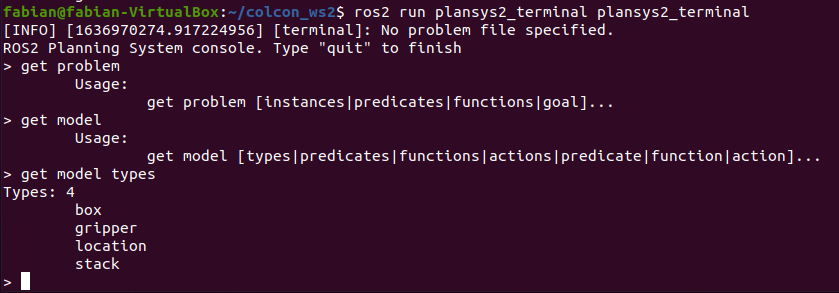
\includegraphics[width=\textwidth]{plansys2terminal}
    \caption{\ac{PlanSys2} Terminal mit Abfrage der Typen des geladenen Models}
    \label{fig:plansysterminal}
\end{figure}

\begin{figure}[ht!]
    \centering
    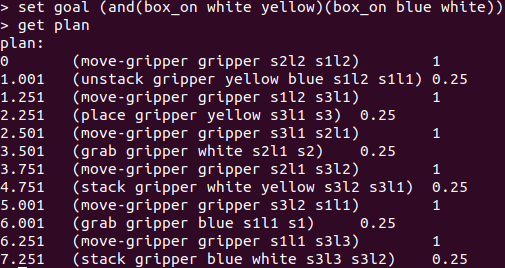
\includegraphics[width=\textwidth]{simple_plan}
    \caption{Ausgabe eines Plans in \ac{PlanSys2} Terminal}
    \label{fig:terminalplan}
\end{figure}